\documentclass[UTF8,zihao=-4,a4paper]{ctexart}
\usepackage{geometry}
\geometry{left=2.6cm,right=2.6cm,top=2.5cm,bottom=2.5cm}
\usepackage{fontspec}
\setmainfont{Times New Roman}
\setCJKmainfont{SimSun}
\usepackage{graphicx}
\usepackage[table]{xcolor}
\usepackage{booktabs}
\usepackage{longtable}
\usepackage{array}
\usepackage{caption}
\usepackage{float}
\usepackage{etoolbox}
\usepackage{fancyhdr}
\usepackage{titlesec}
\usepackage{hyperref}
\hypersetup{colorlinks=true, linkcolor=black, urlcolor=black}
\definecolor{titleblue}{HTML}{1F4E79}
\definecolor{tablehead}{HTML}{ECF6EA}
\definecolor{tableyellow}{HTML}{FFFBEA}
\definecolor{tableline}{HTML}{B6D7A8}
\pagestyle{fancy}
\fancyhf{}
\fancyhead[C]{足球联赛购票系统需求分析与系统详细设计书}
\fancyfoot[C]{\thepage}
\renewcommand{\headrulewidth}{0.4pt}
\setlength{\headheight}{15pt}
\setlength{\parindent}{2em}
\setlength{\parskip}{0.35em}
\linespread{1.25}
\renewcommand{\arraystretch}{1.35}
\titleformat{\section}{\Large\bfseries\color{titleblue}}{}{0pt}{}
\titleformat{\subsection}{\large\bfseries}{}{0pt}{}
\titleformat{\subsubsection}{\normalsize\bfseries}{}{0pt}{}
\captionsetup{font=small,labelfont=bf}
\AtBeginEnvironment{longtable}{\arrayrulecolor{tableline}}
\AtEndEnvironment{longtable}{\arrayrulecolor{black}}
\newcommand{\tablecaptionline}[1]{\vspace{-1.6em}\begin{center}\small\bfseries #1\end{center}\vspace{0.2em}}
\setcounter{tocdepth}{3}
\renewcommand{\contentsname}{目录}
\begin{document}
\begin{center}
{\zihao{2}\bfseries\color{titleblue} 足球联赛购票系统需求分析与系统详细设计书}\\[1.5em]
\end{center}

\begin{center}
{\Large\bfseries\color{titleblue} 摘要}
\end{center}

足球联赛购票系统的设计灵感来源于英超等采用主客场双循环赛制的职业足球联赛。本项目将“找比赛、看球队、买门票”和“俱乐部报名、赛程生成、赛果确认、后台审核”放在同一个业务系统中，形成一套适合课程演示的联赛购票流程。系统面向普通用户、俱乐部负责人、赛事管理员和系统管理员四类角色，不设置独立检票员角色。

本系统的核心功能包括手机号登录、身份选择、预填购票人管理、赛季赛程浏览、俱乐部信息查看、VIP/普通票购买、订单支付、电子票查看、自动退票、俱乐部资料维护、人员管理、赛季报名、赛程确认、赛果录入、赛果审核、营收统计和内部账号管理。购票环节中，用户只选择 VIP 或普通票和购票张数，系统根据 8 个票区的座位结构自动分配座位，并尽量满足同排连坐；赛事和管理环节中，系统通过统一演示时间、角色权限、报名规则和赛果多人确认机制，保证联赛从报名到比赛结束的流程能够完整展示。

\newpage
\tableofcontents
\newpage

\section*{1 系统需求}
\phantomsection
\addcontentsline{toc}{section}{1 系统需求}

\subsection*{1.1 功能需求}
\phantomsection
\addcontentsline{toc}{subsection}{1.1 功能需求}

\subsubsection*{1.1.1 系统角色及其功能}
\phantomsection
\addcontentsline{toc}{subsubsection}{1.1.1 系统角色及其功能}

本系统围绕一场联赛从俱乐部报名、赛程安排、比赛售票到赛果发布的过程展开，因此角色划分也按业务责任来确定。普通用户负责浏览和购票，俱乐部负责人负责维护球队并报名参赛，赛事管理员负责组织赛季和维护赛果，系统管理员负责账号、内部人员、俱乐部和争议赛果的管理。各角色的定位和功能概括如下表所示。


\begin{center}
\small
\begin{longtable}{>{\raggedright\arraybackslash}p{0.17\textwidth} >{\raggedright\arraybackslash}p{0.31\textwidth} >{\raggedright\arraybackslash}p{0.44\textwidth}}
\toprule
\rowcolor{tablehead}
\textbf{角色} & \textbf{说明} & \textbf{主要功能} \\
\midrule
\endfirsthead
\toprule
\rowcolor{tablehead}
\textbf{角色} & \textbf{说明} & \textbf{主要功能} \\
\midrule
\endhead
普通用户 & 观赛与购票用户 & 注册登录、账号资料、预填购票人、比赛浏览、购票支付、电子票、订单退票 \\
\midrule
俱乐部负责人 & 负责俱乐部资料和报名 & 俱乐部资料、队徽上传、主场信息、人员管理、赛季报名、赛程查看、俱乐部数据 \\
\midrule
赛事管理员 & 负责赛季和赛果管理 & 创建赛季、处理报名、确认赛程、发布比赛、维护比分、赛季营收、平台分成 \\
\midrule
系统管理员 & 负责后台基础管理 & 用户管理、内部人员管理、俱乐部管理、负责人审核、争议赛果审核、系统参数 \\
\midrule
\bottomrule
\end{longtable}
\end{center}

\tablecaptionline{表 1-1 系统角色说明表}

\subsubsection*{1.1.2 需求规定}
\phantomsection
\addcontentsline{toc}{subsubsection}{1.1.2 需求规定}

在需求规定上，本系统主要围绕两个方向展开：用户端完成购票流程，后台完成赛事、票务、俱乐部和账号管理。系统不追求覆盖真实票务平台的所有复杂情况，但需要完整表现一场比赛从发布、售票、下单、支付到退票的主要过程。


\begin{center}
\small
\begin{longtable}{>{\raggedright\arraybackslash}p{0.17\textwidth} >{\raggedright\arraybackslash}p{0.31\textwidth} >{\raggedright\arraybackslash}p{0.44\textwidth}}
\toprule
\rowcolor{tablehead}
\textbf{编号} & \textbf{功能} & \textbf{功能规定} \\
\midrule
\endfirsthead
\toprule
\rowcolor{tablehead}
\textbf{编号} & \textbf{功能} & \textbf{功能规定} \\
\midrule
\endhead
F01 & 注册与登录 & 普通用户和俱乐部负责人可注册；赛事管理员和系统管理员由已有系统管理员内部登记；登录时选择身份，管理员需填写工号 \\
\midrule
F02 & 比赛与球队浏览 & 查看赛季、轮次、积分榜、比赛详情、场馆和双方俱乐部信息 \\
\midrule
F03 & 俱乐部报名 & 报名期内提交报名；检查赛季时间、报名冲突、主场、球员和教练信息 \\
\midrule
F04 & 赛程与比赛管理 & 创建赛季、生成主客场双循环赛程、发布比赛、维护比分 \\
\midrule
F05 & 票务管理 & 票区由主场信息生成；用户端只区分 VIP 和普通票；售票和退票时间自动计算 \\
\midrule
F06 & 购票与支付 & 选择票种、张数和等量购票人；系统限制张数并尽量分配同排连坐；支付后生成电子票 \\
\midrule
F07 & 自动退票 & 用户在订单中申请；系统按开赛时间计算退款比例，更新订单、电子票和座位状态 \\
\midrule
F08 & 统计与时间 & 营收、平台分成、俱乐部收益、胜负场、积分、净胜球统计；支持调整演示时间 \\
\midrule
\bottomrule
\end{longtable}
\end{center}

\tablecaptionline{表 1-2 功能需求规定表}

系统设置了不同的注册和登录要求：普通用户可直接注册登录；俱乐部负责人注册后需要审核；赛事管理员和系统管理员由已有系统管理员内部先行注册。登录时需要选择身份，管理人员还要填写工号。

\subsubsection*{1.1.3 业务流程概述}
\phantomsection
\addcontentsline{toc}{subsubsection}{1.1.3 业务流程概述}

系统初始化时保留一个系统管理员账号，用于进入后台并登记新的赛事管理员和系统管理员。内部管理员账号由系统管理员预先登记手机号、姓名和工号，账号初始为“注册中”状态；本人首次登录时需要校验手机号、姓名和工号，设置密码后才正式启用。普通用户和俱乐部负责人可以公开注册，其中俱乐部负责人注册后需要等待审核。若审核尚未通过，系统应明确提示“俱乐部审核中，请先以普通用户身份进入”，避免只显示“无权限”造成误解。

赛事管理员创建赛季时只填写赛季开始日期和参赛队伍上限，系统按主客场双循环规则计算赛季持续时间，并在报名截止或达到队伍上限后生成赛程。生成后的赛程由赛事管理员确认，确认后才进入比赛发布和售票流程。俱乐部负责人报名赛季前，需要先维护俱乐部资料、主场结构、球员和教练信息；报名提交时系统保存当次报名阵容快照，后续球队人员调整不影响已经报名成功的赛季阵容。

比赛发布后，系统根据统一演示时间自动控制报名、开售、停售和退票规则。用户在比赛详情中查看赛季、轮次、比赛时间、剩余票数、场馆地址、双方俱乐部、VIP/普通票价和余票；球队名称和队徽都可以作为进入俱乐部详情的入口。未开售时页面只提示开售时间，已开售后重点展示票价和余票，不展示停售时间、票总数、场馆结构、座位范围或最大连坐数等偏后台信息。

用户购票时从预填购票人中选择出票人，再选择 VIP 或普通票和购票张数。购票人数必须与购票张数一致，例如购买 3 张票时必须选择 3 名购票人。若购票人不足，用户可以在购票人选择区域直接新增；门票尚未开售时，用户也可以提前维护预填购票人，等到开售时间后直接开始购买。系统根据余票限制可选张数，并在对应票种的多个方向票区中自动安排座位，优先保证同排连坐；若完整连坐无法满足，再提示系统将尽量分配连坐座位。订单创建后暂时锁定座位，支付成功后生成电子票；订单取消、超时或自动退票后，座位重新释放。

上述业务流程在正式文档中配四张角色流程图展示，分别对应普通用户、俱乐部负责人、赛事管理员和系统管理员。下方流程图用于概括各角色从进入系统到完成核心业务的主要路径。

\begin{figure}[H]
\centering
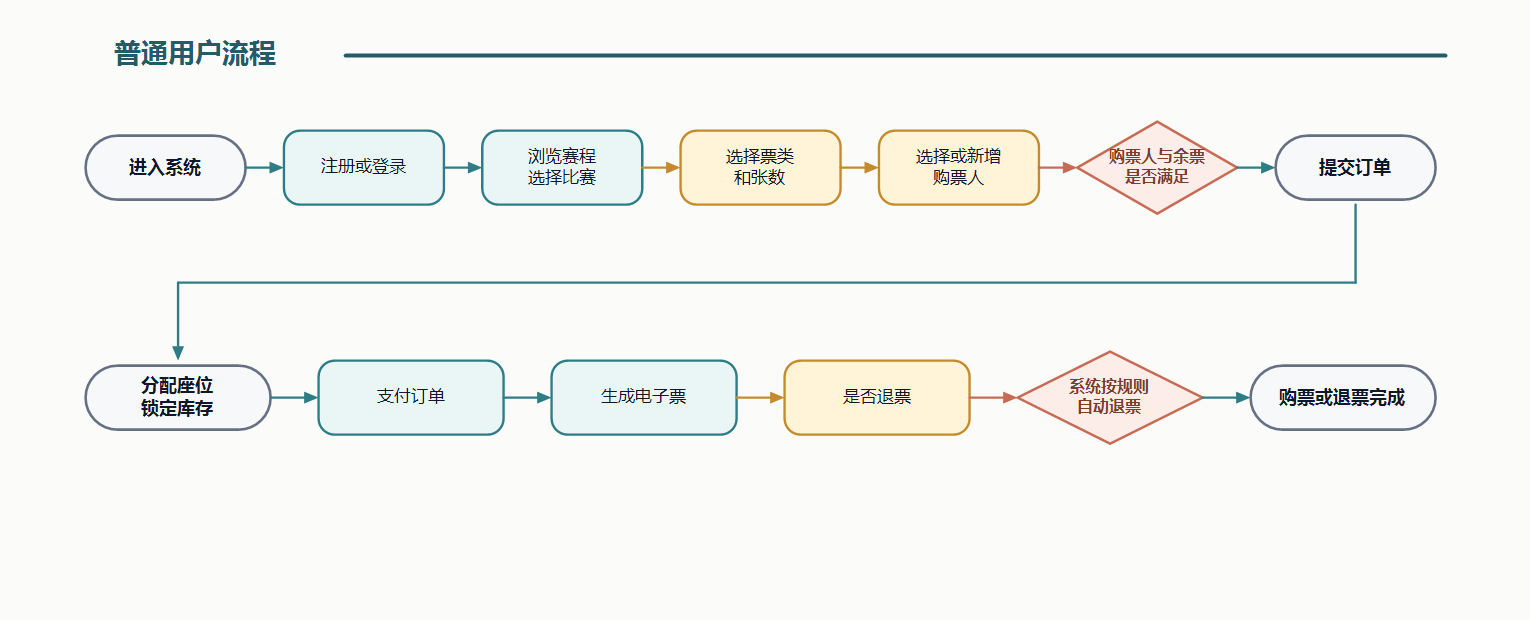
\includegraphics[width=0.96\textwidth]{figures/user.png}
\caption*{图 1-1 普通用户购票与退票流程图}
\end{figure}

\begin{figure}[H]
\centering
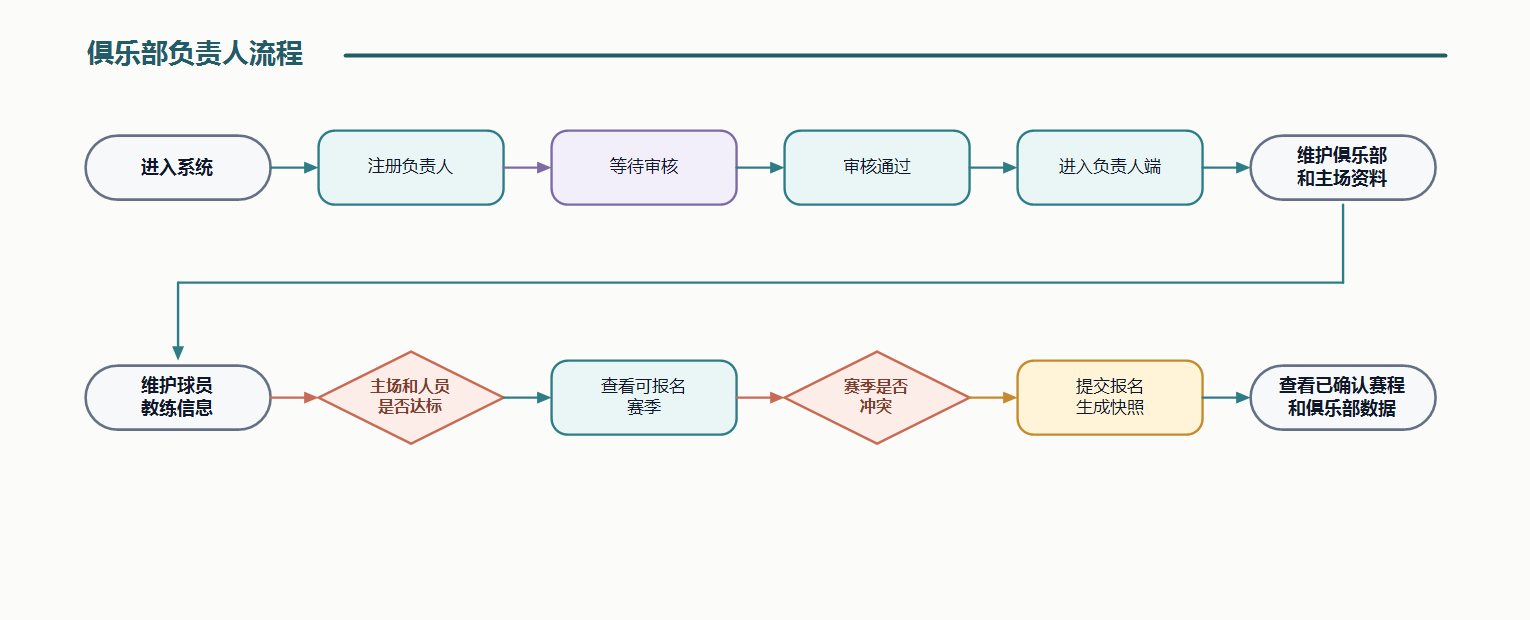
\includegraphics[width=0.96\textwidth]{figures/club.png}
\caption*{图 1-2 俱乐部负责人赛季报名与收入查看流程图}
\end{figure}

\begin{figure}[H]
\centering
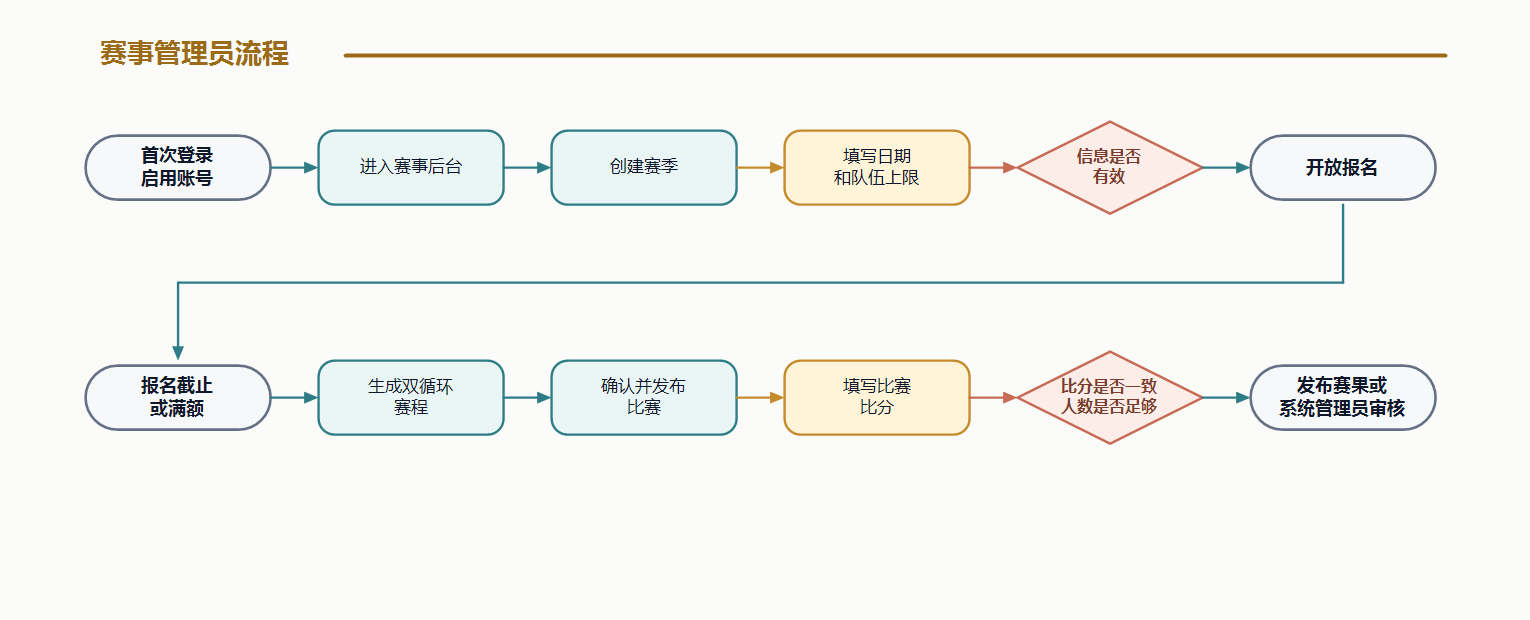
\includegraphics[width=0.96\textwidth]{figures/match.png}
\caption*{图 1-3 赛事管理员赛季创建与赛果维护流程图}
\end{figure}

\begin{figure}[H]
\centering
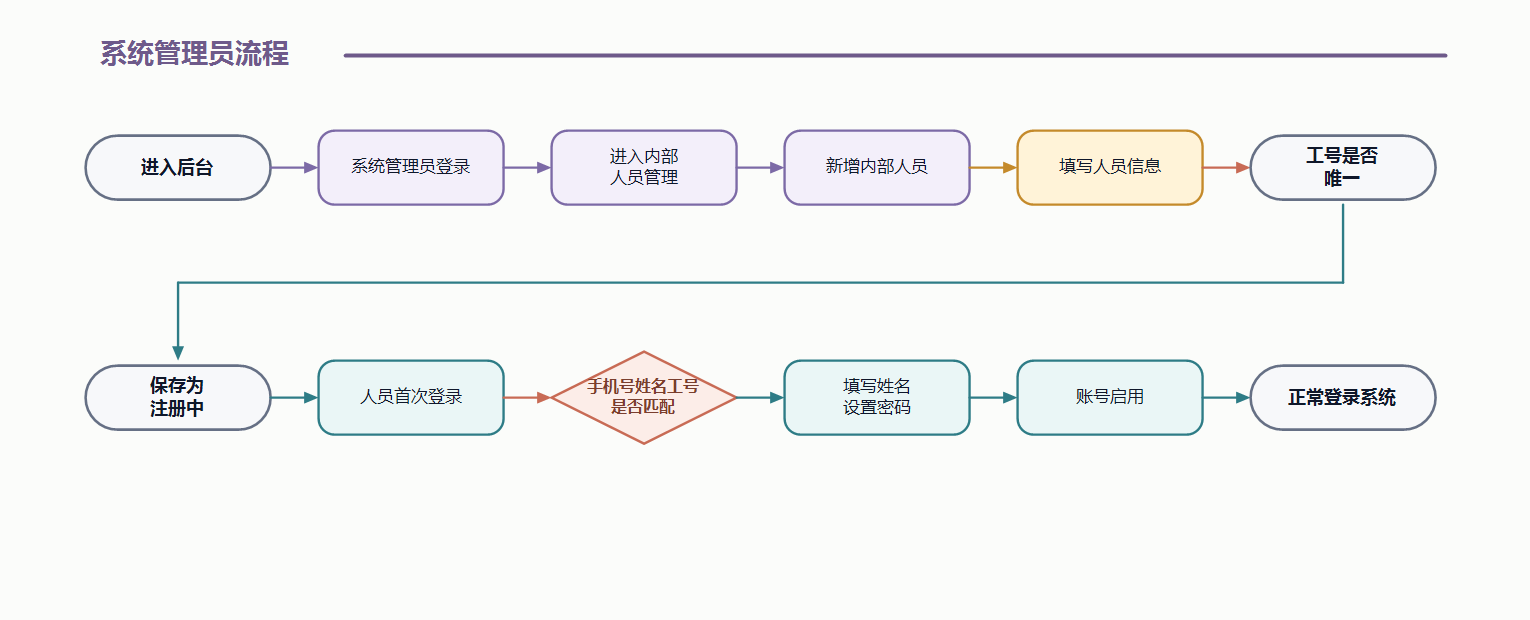
\includegraphics[width=0.96\textwidth]{figures/system.png}
\caption*{图 1-4 系统管理员内部人员注册与启用流程图}
\end{figure}

为了方便课堂演示，系统不直接依赖电脑真实时间，而是设计统一的业务当前时间。四类角色均可调整该时间，报名开放、售票开放、退票比例、比赛状态和赛果录入限制都以该时间为准。

考虑到本次课程设计重点在联赛组织与购票流程，当前版本不设置独立检票角色。电子票主要作为用户查看购票结果和订单状态的凭证，退票操作统一收口到“我的订单”中完成。

\subsubsection*{1.1.4 业务实体分析}
\phantomsection
\addcontentsline{toc}{subsubsection}{1.1.4 业务实体分析}

根据上述需求，系统涉及的主要实体包括账号、角色、预填购票人、内部人员登记、俱乐部、球员、教练、赛季、报名、报名阵容快照、轮次、比赛、场馆、票区、座位、订单、支付记录、电子票、退票记录和赛果审核记录。这些实体基本覆盖了本课题需要处理的业务对象。


\begin{center}
\small
\begin{longtable}{>{\raggedright\arraybackslash}p{0.17\textwidth} >{\raggedright\arraybackslash}p{0.31\textwidth} >{\raggedright\arraybackslash}p{0.44\textwidth}}
\toprule
\rowcolor{tablehead}
\textbf{实体} & \textbf{主要内容} & \textbf{说明} \\
\midrule
\endfirsthead
\toprule
\rowcolor{tablehead}
\textbf{实体} & \textbf{主要内容} & \textbf{说明} \\
\midrule
\endhead
账号与角色 & 账号、手机号、密码、身份、工号、状态 & 登录、权限判断、后台账号管理 \\
\midrule
购票人与订单 & 预填购票人、订单、支付记录、电子票 & 购票人选择、订单支付、出票 \\
\midrule
俱乐部与人员 & 俱乐部、负责人、球员、教练、报名阵容快照 & 球队展示、赛季报名、俱乐部管理 \\
\midrule
赛季与比赛 & 赛季、轮次、主队、客队、比赛时间、比分提交、赛果审核 & 联赛组织、赛程展示、赛果确认 \\
\midrule
场馆与票区 & 场馆、区域、座位、票价、库存 & 比赛售票、座位分配 \\
\midrule
退票与日志 & 退票记录、退款规则、系统时间配置、操作记录 & 自动退票、演示时间管理、系统维护 \\
\midrule
\bottomrule
\end{longtable}
\end{center}

\tablecaptionline{表 1-3 业务实体说明表}

登录失败时，系统应给出清楚提示，例如账号未注册、密码错误、身份不匹配或工号不正确，让用户知道问题出在哪里。

\subsubsection*{1.1.5 需求补充说明}
\phantomsection
\addcontentsline{toc}{subsubsection}{1.1.5 需求补充说明}

正式功能只保留普通用户、俱乐部负责人、赛事管理员和系统管理员四类角色。注册页面面向普通用户和俱乐部负责人开放；赛事管理员和系统管理员不开放自行注册，只能由已有系统管理员在“内部人员管理”中预先登记。登记时填写管理员类型、手机号、姓名和 4 位工号数字，系统按类型自动拼接 EA 或 SA 前缀。

同一个手机号可以在符合规则的情况下注册多个不同身份，因此系统内部仍需要保留账号 ID、身份、手机号和必要工号来区分账号；但账号 ID 只作为内部标识，不在前端页面展示。用户可见文案统一使用“用户名”，不再使用“昵称”；手机号作为登录凭证和账号绑定信息展示，不允许用户自行修改。

账号资料不作为一级栏目出现，而是通过点击右上角头像或用户名进入下拉菜单，再访问账号资料、切换账户或退出登录。切换账户应进入单独界面，不与退出登录混成同一个动作。普通用户注册不要求填写真实姓名，购票实名信息改为单独维护“预填购票人”：同一用户最多维护 4 个购票人，同一个购票人最多被不同用户预填 4 次，删除后释放对应名额。

俱乐部负责人注册时提交的俱乐部信息先形成俱乐部注册申请，系统管理员审核通过后，该申请转为正式俱乐部并与负责人账号绑定。系统不提供“关联已有俱乐部”的注册方式，保证一个俱乐部有且仅有一个负责人；系统初始化和演示数据中也不应出现无负责人的正式俱乐部。俱乐部状态、账号状态等页面文案统一使用“已启用”“已停用”等中文表述，不直接向用户展示 ACTIVE、ENABLED 等后台状态值。

\subsection*{1.2 非功能性需求}
\phantomsection
\addcontentsline{toc}{subsection}{1.2 非功能性需求}


\begin{center}
\small
\begin{longtable}{>{\raggedright\arraybackslash}p{0.22\textwidth} >{\raggedright\arraybackslash}p{0.70\textwidth}}
\toprule
\rowcolor{tablehead}
\textbf{类别} & \textbf{需求说明} \\
\midrule
\endfirsthead
\toprule
\rowcolor{tablehead}
\textbf{类别} & \textbf{需求说明} \\
\midrule
\endhead
性能需求 & 常规查询响应控制在 2 秒以内；购票高峰避免超卖和长时间等待 \\
\midrule
安全需求 & 密码加密存储；后台按角色鉴权；电子票码唯一且不可重复使用 \\
\midrule
可靠性需求 & 支付、库存扣减、电子票生成保持一致；异常后订单状态可恢复 \\
\midrule
易用性需求 & 比赛浏览、购票张数、订单确认和电子票查看流程清晰；用户无需手动选座 \\
\midrule
可维护性需求 & 采用 MVC 分层结构；控制层、业务层、数据访问层和前端展示层分离 \\
\midrule
兼容性需求 & 用户端适配桌面和移动端浏览器；后台优先保证桌面端操作效率 \\
\midrule
\bottomrule
\end{longtable}
\end{center}

\tablecaptionline{表 1-4 非功能性需求表}

\section*{2 系统设计}
\phantomsection
\addcontentsline{toc}{section}{2 系统设计}

\subsection*{2.1 系统总体架构设计}
\phantomsection
\addcontentsline{toc}{subsection}{2.1 系统总体架构设计}

系统采用前后端分离结构，按使用者分为用户端、俱乐部负责人端、赛事管理端和系统管理端。用户端主要面向比赛浏览、购票、订单和电子票；俱乐部负责人端主要面向俱乐部资料、人员管理、赛季报名和俱乐部数据；赛事管理端主要面向赛季创建、报名处理、赛程确认、比赛发布和赛果维护；系统管理端主要面向用户管理、内部人员管理、俱乐部管理和争议赛果审核。后端按 MVC 思想分层，数据库使用 MySQL 保存业务数据。

技术结构分为表示层、控制层、业务逻辑层、数据访问层和数据库层，符合课程设计对多层架构的要求。


\begin{center}
\small
\begin{longtable}{>{\raggedright\arraybackslash}p{0.17\textwidth} >{\raggedright\arraybackslash}p{0.31\textwidth} >{\raggedright\arraybackslash}p{0.44\textwidth}}
\toprule
\rowcolor{tablehead}
\textbf{技术层次} & \textbf{主要职责} & \textbf{使用技术} \\
\midrule
\endfirsthead
\toprule
\rowcolor{tablehead}
\textbf{技术层次} & \textbf{主要职责} & \textbf{使用技术} \\
\midrule
\endhead
表示层 & 用户端、俱乐部负责人端、赛事管理员后台、系统管理员后台 & Vue、Element Plus、Axios \\
\midrule
控制层 & 接收请求、参数校验、登录鉴权、接口响应封装 & Spring MVC Controller \\
\midrule
业务逻辑层 & 认证授权、系统时间、俱乐部审核、赛季报名、赛程生成、连坐规划、库存锁定、订单支付、电子票、自动退票、赛果维护 & Spring Boot Service \\
\midrule
数据访问层 & 账号、俱乐部、赛季、比赛、座位、订单、支付、退票和统计数据访问 & MyBatis Mapper \\
\midrule
数据层 & 存储核心业务数据；通过事务保证订单、库存、电子票和退票状态一致 & MySQL \\
\midrule
\bottomrule
\end{longtable}
\end{center}

\tablecaptionline{表 2-1 技术分层设计表}

系统整体流程为：用户通过前端页面访问系统，后端完成业务处理和权限判断，数据库保存账号、赛事、票务和订单等数据。

\subsection*{2.2 功能模块设计}
\phantomsection
\addcontentsline{toc}{subsection}{2.2 功能模块设计}

\subsubsection*{2.2.1 功能模块划分}
\phantomsection
\addcontentsline{toc}{subsubsection}{2.2.1 功能模块划分}

系统功能可以划分为账号、赛事、俱乐部、票务和统计五类。账号模块负责注册、登录、身份选择、工号校验、账号资料和账号启停；赛事模块负责赛季、报名、轮次、比赛、比分和积分榜；俱乐部模块负责俱乐部资料、队徽、主场信息、球员、教练、报名阵容快照和俱乐部数据；票务模块负责 VIP/普通票、8 个票区、座位库存、下单锁定、支付、电子票和自动退票；统计模块负责售票数、销售额、退款金额、平台分成、俱乐部收益、胜负场、积分、净胜球和排行榜。

\subsubsection*{2.2.2 赛季报名与赛程功能点设计}
\phantomsection
\addcontentsline{toc}{subsubsection}{2.2.2 赛季报名与赛程功能点设计}

俱乐部负责人通过审核后，可以在报名期内提交赛季报名。报名时需要保证本俱乐部资料完整，并且没有与目标赛季冲突的报名记录。

报名信息包括俱乐部、主场、球员和教练。系统会检查人员和主场是否满足比赛要求：当前阵容必须有且仅有 1 名首发门将、刚好 11 名首发球员、替补不超过 7 人，并且有且仅有 1 名现役主教练、至多 2 名现役副教练；主场必须填写每区排数、长边每排座位数和宽边每排座位数。

报名结束后，赛事管理员可生成主客场双循环赛程。生成后由赛事管理员检查和确认，再进入比赛发布和票务配置环节。

\subsubsection*{2.2.3 购票功能点设计}
\phantomsection
\addcontentsline{toc}{subsubsection}{2.2.3 购票功能点设计}

购票功能主要包括选择比赛、选择 VIP 或普通票、选择购票人、提交订单、模拟支付和查看电子票。用户不需要手动选择具体方向或具体座位，座位由系统根据票种、购票张数和主场座位布局自动安排。

购票时，系统会检查比赛状态、销售时间、余票、购票数量和购票人数量。页面只突出展示票价和余票数；未开售时显示开售时间，已开售后不再常驻展示开售时间。最大连坐数不直接展示给用户，只有当用户选择的张数无法满足完整连坐时，才提示“系统无法满足连坐需求，将为您尽量分配连坐座位”。符合条件后生成订单并锁定座位，支付成功后再正式出票。

\subsubsection*{2.2.4 比赛结果与退票规则说明}
\phantomsection
\addcontentsline{toc}{subsubsection}{2.2.4 比赛结果与退票规则说明}

比赛结果由赛事管理员维护，未到比赛日期时不能录入比分。若有多个赛事管理员，同一场比赛至少需要 2 人录入完全相同比分后才自动发布；若比分不一致或只有 1 人录入，则交由系统管理员进行赛果审核。比分主要用于比赛展示、积分榜、排行榜和后续统计。

退票不需要管理员审核，系统按照比赛开始时间自动判断退款比例。开赛前 7 天以外退票全额退款，开赛前 7 天内退票收取 50\% 手续费；每场比赛开赛前 1 小时停止售票。


\begin{center}
\small
\begin{longtable}{>{\raggedright\arraybackslash}p{0.20\textwidth} >{\raggedright\arraybackslash}p{0.38\textwidth} >{\raggedright\arraybackslash}p{0.34\textwidth}}
\toprule
\rowcolor{tablehead}
\textbf{业务内容} & \textbf{规则} & \textbf{处理结果} \\
\midrule
\endfirsthead
\toprule
\rowcolor{tablehead}
\textbf{业务内容} & \textbf{规则} & \textbf{处理结果} \\
\midrule
\endhead
比分录入 & 比赛日期已到后可录入比分；未到比赛日期不能提前录入 & 用于比赛结果、积分榜、排行榜和俱乐部数据统计 \\
\midrule
赛果发布 & 多名赛事管理员录入同一比分时自动发布；比分冲突或仅 1 人录入时交由系统管理员审核 & 审核通过后形成正式赛果 \\
\midrule
自动退票 & 用户在订单中申请退票；系统按比赛时间计算退款金额并释放库存 & 开赛前 7 天以外全额退款，7 天内收取 50\% 手续费 \\
\midrule
\bottomrule
\end{longtable}
\end{center}

\tablecaptionline{表 2-2 比赛结果与退票规则表}

比分维护影响比赛结果、积分、净胜球和排行榜；退票处理影响订单、电子票、座位库存和营收统计，两类业务分别记录。

\subsection*{2.3 数据库设计}
\phantomsection
\addcontentsline{toc}{subsection}{2.3 数据库设计}

\subsubsection*{2.3.1 逻辑结构设计}
\phantomsection
\addcontentsline{toc}{subsubsection}{2.3.1 逻辑结构设计}

数据库设计围绕“人、队、赛、票、单”几条主线展开。账号数据需要支持同一手机号注册多个身份，俱乐部数据需要保存负责人和报名阵容快照，票务数据需要支持 8 个票区、座位锁定和自动退票，赛果数据还需要记录多名赛事管理员提交的比分和系统管理员审核结果。主要关系如下表所示：


\begin{center}
\small
\begin{longtable}{>{\raggedright\arraybackslash}p{0.22\textwidth} >{\raggedright\arraybackslash}p{0.70\textwidth}}
\toprule
\rowcolor{tablehead}
\textbf{主线} & \textbf{主要关系} \\
\midrule
\endfirsthead
\toprule
\rowcolor{tablehead}
\textbf{主线} & \textbf{主要关系} \\
\midrule
\endhead
账号 & 账号 $\rightarrow$ 身份 $\rightarrow$ 权限 $\rightarrow$ 个人资料或后台功能 \\
\midrule
俱乐部 & 俱乐部负责人 $\rightarrow$ 俱乐部 $\rightarrow$ 主场信息 $\rightarrow$ 球员/教练 $\rightarrow$ 赛季报名快照 \\
\midrule
赛事 & 赛季 $\rightarrow$ 报名 $\rightarrow$ 轮次 $\rightarrow$ 比赛 $\rightarrow$ 比分提交/赛果审核 \\
\midrule
票务 & 比赛 $\rightarrow$ VIP/普通票区 $\rightarrow$ 座位库存 $\rightarrow$ 座位锁定 $\rightarrow$ 订单 \\
\midrule
交易 & 预填购票人 $\rightarrow$ 订单 $\rightarrow$ 支付记录 $\rightarrow$ 电子票 $\rightarrow$ 自动退票记录 \\
\midrule
\bottomrule
\end{longtable}
\end{center}

\tablecaptionline{表 2-3 数据库主要关系表}

账号表保存手机号、密码、身份、工号、状态和内部账号 ID。手机号用于登录，但不能单独作为账号唯一依据；系统需要结合身份、手机号以及管理员工号区分不同账号。管理员账号还需要保存预登记信息和首次启用状态，用来支持“系统管理员先登记、本人首次登录启用”的流程。

俱乐部表保存俱乐部名称、队徽、城市、负责人和启停状态。主场信息由俱乐部负责人维护，包含场馆名称、地址、VIP/普通价格、每区排数、长边每排座位数和宽边每排座位数。系统根据这些数据生成东西南北 4 个方向、每个方向 VIP 和普通 2 类区域的 8 个票区结构。

人员数据分为球员和教练。球员保存姓名、出生年份、国籍、位置、球衣号和首发/替补/离队状态；教练保存姓名、出生年份、国籍、主教练/副教练职务和现役/离队状态。报名成功时需要把当时的人员和主场信息保存为报名快照，防止后续球队调整影响已经报名的赛季。

订单与票务数据需要同时记录购票人、票种、座位、订单状态、支付状态和电子票状态。下单时先锁定座位，支付成功后生成电子票；订单取消、超时或退票成功时释放座位。自动退票记录保存退款比例、手续费和退款金额，用于后续营收统计。

\subsubsection*{2.3.2 物理结构设计}
\phantomsection
\addcontentsline{toc}{subsubsection}{2.3.2 物理结构设计}


\begin{center}
\small
\begin{longtable}{>{\raggedright\arraybackslash}p{0.17\textwidth} >{\raggedright\arraybackslash}p{0.31\textwidth} >{\raggedright\arraybackslash}p{0.44\textwidth}}
\toprule
\rowcolor{tablehead}
\textbf{类别} & \textbf{主要表或数据} & \textbf{用途} \\
\midrule
\endfirsthead
\toprule
\rowcolor{tablehead}
\textbf{类别} & \textbf{主要表或数据} & \textbf{用途} \\
\midrule
\endhead
账号权限 & 账号表、角色表、内部人员登记表、权限表 & 账号 ID、手机号、身份、工号、状态、首次启用信息、角色权限 \\
\midrule
俱乐部 & 俱乐部表、主场表、球员表、教练表、报名表、报名阵容快照表 & 俱乐部资料、负责人绑定、场馆结构、人员信息、报名快照 \\
\midrule
赛事 & 赛季表、轮次表、比赛表、排赛批次表、比分提交表、赛果审核表 & 赛季规则、赛程、比赛时间、主客队、比分提交、最终赛果 \\
\midrule
场馆票务 & 场馆表、票区表、座位表、比赛库存表、座位锁定表 & 8 个票区、VIP/普通价格、余票、座位状态、下单锁定信息 \\
\midrule
订单支付 & 预填购票人表、订单表、订单明细表、支付记录表、电子票表 & 购票人、购票订单、支付结果、座位快照、电子票码 \\
\midrule
退票统计 & 退票记录表、退款记录表、系统时间配置表、操作日志表、营收统计表 & 自动退票结果、业务当前时间、操作记录、营收分成数据 \\
\midrule
\bottomrule
\end{longtable}
\end{center}

\tablecaptionline{表 2-4 物理结构设计表}

\subsection*{2.4 关键业务规则设计}
\phantomsection
\addcontentsline{toc}{subsection}{2.4 关键业务规则设计}


\begin{center}
\small
\begin{longtable}{>{\raggedright\arraybackslash}p{0.22\textwidth} >{\raggedright\arraybackslash}p{0.70\textwidth}}
\toprule
\rowcolor{tablehead}
\textbf{规则} & \textbf{说明} \\
\midrule
\endfirsthead
\toprule
\rowcolor{tablehead}
\textbf{规则} & \textbf{说明} \\
\midrule
\endhead
角色权限 & 四类角色使用不同功能；赛事管理员和系统管理员可统称管理员，系统内部仍按具体身份授权 \\
\midrule
注册登录 & 普通用户和俱乐部负责人可公开注册；管理员由系统管理员内部预登记，首次登录校验手机号、姓名和工号 \\
\midrule
俱乐部审核 & 负责人注册后需审核；审核通过后创建俱乐部并绑定负责人；一个俱乐部有且仅有一个负责人 \\
\midrule
赛季报名 & 报名必须在开放期内；主场、场地结构、球员和教练信息需符合参赛规则；报名后保存阵容快照 \\
\midrule
自动开售 & 报名截止次日 20:00 开售；比赛开赛前 1 小时停售；时间判断使用统一演示时间 \\
\midrule
购票支付 & 单笔最多 4 张；用户只选 VIP 或普通票；购票人数量等于购票张数；系统尽量分配同排连坐 \\
\midrule
退票 & 用户在订单中申请；开赛前 7 天以外全额退款，7 天内收取 50\% 手续费；系统自动更新状态 \\
\midrule
赛果确认 & 多名赛事管理员提交相同比分后自动发布；比分冲突或提交人数不足时由系统管理员审核 \\
\midrule
数据安全 & 密码加密保存；后台接口按角色鉴权；座位锁定和库存扣减保持一致；关键操作保留记录 \\
\midrule
\bottomrule
\end{longtable}
\end{center}

\tablecaptionline{表 2-5 关键业务规则表}

\subsection*{2.5 界面设计说明}
\phantomsection
\addcontentsline{toc}{subsection}{2.5 界面设计说明}

界面包括登录注册页、普通用户页面、俱乐部负责人页面、赛事管理员页面和系统管理员页面。各角色页面的一级导航位置应保持一致，避免同一系统在不同身份下出现明显不同的布局逻辑。前端展示文案应面向最终用户，不显示“阶段几”、ACTIVE、ENABLED 等开发或数据库枚举用语。

普通用户页面重点展示赛季赛程、比赛详情、球队信息、VIP/普通票价、余票、订单和电子票。账号资料入口放在头像或用户名下拉菜单中，不作为一级栏目；退票入口收口到“我的订单”，电子票页面默认展示未使用票，不重复展示已退票分类。

俱乐部负责人页面重点展示俱乐部资料、人员管理、赛季报名、已确认赛程和俱乐部数据。人员管理作为一级入口，下设球员管理和教练管理，人员总览页只展示当前首发、替补和现役教练，并集中显示参赛合规提醒。赛事管理员页面重点展示赛季创建、报名处理、赛程确认、比赛发布、赛果维护和营收统计；系统管理员页面重点拆分为用户管理、内部人员管理和俱乐部管理，并增加争议赛果审核。

\section*{3 未来展望}
\phantomsection
\addcontentsline{toc}{section}{3 未来展望}

在当前版本之外，系统还保留了几项后续可扩展功能。以下内容不作为本次必须实现范围，只作为以后继续完善系统时的方向，避免被误认为当前版本需要立刻完成的功能。

\subsection*{3.1 比赛互动功能}
\phantomsection
\addcontentsline{toc}{subsection}{3.1 比赛互动功能}

比赛详情页后续可以增加赛前胜负预测投票。用户在比赛开始前选择支持主队或客队，系统展示双方支持率。这个功能主要用于增加观赛互动，不影响比赛结果、购票资格和座位分配。

\subsection*{3.2 热门比赛购票稳定性}
\phantomsection
\addcontentsline{toc}{subsection}{3.2 热门比赛购票稳定性}

热门比赛开售时可能会有较多用户同时下单。后续可以在座位锁定、订单创建和库存扣减中加入更完整的并发控制，避免两名用户在同一时间买到同一张票。

\subsection*{3.3 球队与球员信息展示}
\phantomsection
\addcontentsline{toc}{subsection}{3.3 球队与球员信息展示}

俱乐部详情页可以继续补充球员赛季数据，例如出场数、进球数、助攻数和牌数等。阵容展示也可以加入更直观的站位图，让用户看到球队大致排布。

\subsection*{3.4 俱乐部长期管理}
\phantomsection
\addcontentsline{toc}{subsection}{3.4 俱乐部长期管理}

俱乐部管理后续可以增加转会等长期管理功能，保留球员在不同赛季和不同俱乐部的历史信息。等到比赛、球员和订单数据积累较多后，也可以尝试加入 AI 比赛预测模型，作为用户观赛前的参考信息。

\section*{4 小结}
\phantomsection
\addcontentsline{toc}{section}{4 小结}

本系统围绕足球联赛购票这一场景，把普通用户买票、俱乐部负责人报名、赛事管理员组织赛季和系统管理员后台审核几个流程串联起来。相比只做普通票务系统，本项目更强调联赛业务本身：俱乐部需要先完善主场和人员信息，赛事管理员按主客场双循环生成赛程，用户在比赛发布后按 VIP 或普通票购票，系统再自动完成座位分配、电子票生成和退票处理。

在设计过程中，较关键的部分包括多身份账号登录、管理员内部预登记、俱乐部一负责人规则、人员参赛合规检查、8 个票区座位模型、同排连坐分配、统一演示时间、自动退票规则和多人赛果确认。数据库设计也围绕这些规则展开，既保存当前业务状态，也保留报名阵容、座位锁定、退款记录和赛果审核等过程数据，便于课程演示时展示完整业务闭环。

\end{document}
